% CARE-U Technical Documentation
% Compile: pdflatex technical-documentation.tex (run twice for TOC)
\documentclass[11pt,a4paper]{report}

\usepackage[utf8]{inputenc}
\usepackage[T1]{fontenc}
\usepackage{lmodern}
\usepackage[margin=2.5cm]{geometry}
\usepackage{graphicx}
\usepackage{hyperref}
\usepackage{listings}
\usepackage{xcolor}
\usepackage{booktabs}
\usepackage{longtable}
\usepackage{enumitem}
\usepackage{tikz}
\usetikzlibrary{shapes,arrows.meta,positioning}

\hypersetup{
    colorlinks=true,
    linkcolor=blue!60!black,
    urlcolor=blue!60!black,
    pdftitle={CARE-U Technical Documentation},
}

\lstdefinestyle{code}{
    basicstyle=\ttfamily\small,
    breaklines=true,
    frame=single,
    backgroundcolor=\color{gray!8},
    keywordstyle=\color{blue!70!black},
    commentstyle=\color{green!40!black},
    stringstyle=\color{red!60!black},
}

\title{\textbf{CARE-U}\\[0.4em]
\large Technical Documentation}
\author{Engineering Team}
\date{\today}

\begin{document}

\maketitle
\tableofcontents
\newpage

%==============================================================================
\chapter{Introduction}
%==============================================================================

\section{Purpose}
This document describes the technical architecture, deployment model, security boundaries, and integration interfaces of \textbf{CARE-U}---a multi-tenant hospital management platform built with Django~5+ and PostgreSQL schema isolation via \texttt{django-tenants}.

\section{Scope}
\begin{itemize}[noitemsep]
    \item Platform architecture and tenant isolation
    \item Application modules and data models
    \item Authentication and authorization
    \item REST API and background tasks
    \item Deployment, configuration, and operations
\end{itemize}

\section{Technology Stack}
\begin{table}[h]
\centering
\begin{tabular}{@{}ll@{}}
\toprule
\textbf{Layer} & \textbf{Technology} \\
\midrule
Backend & Django 5.1+, Python 3.11+ \\
Multi-tenancy & django-tenants (PostgreSQL schemas) \\
API & Django REST Framework, JWT (SimpleJWT) \\
Database & PostgreSQL (production), SQLite (dev) \\
Cache / queue & Redis, Celery, Celery Beat \\
Real-time & Django Channels, Daphne \\
Frontend UI & Django templates, Tailwind CSS, Alpine.js \\
Documentation API & drf-spectacular (OpenAPI) \\
\bottomrule
\end{tabular}
\caption{Core technology stack}
\end{table}

%==============================================================================
\chapter{System Architecture}
%==============================================================================

\section{Multi-Tenant Model}

Each registered hospital receives:
\begin{enumerate}[noitemsep]
    \item A dedicated \textbf{PostgreSQL schema} (e.g.\ \texttt{gph\_islamabad})
    \item A \textbf{subdomain / subfolder} route: \texttt{/h/\{subdomain\}/}
    \item An isolated copy of all tenant-scoped ERP tables
\end{enumerate}

The \textbf{public schema} holds platform-wide data only.

\begin{figure}[h]
\centering
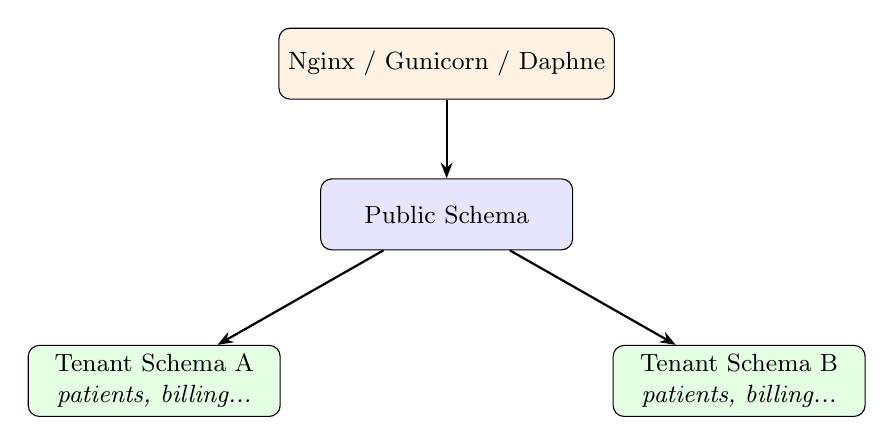
\begin{tikzpicture}[
    box/.style={draw, rounded corners, minimum width=3.2cm, minimum height=0.9cm, align=center, font=\small},
    arr/.style={-{Stealth[length=2mm]}, thick}
]
    \node[box, fill=blue!10] (pub) {Public Schema};
    \node[box, fill=green!10, below left=1.2cm and 0.5cm of pub] (t1) {Tenant Schema A\\ \textit{patients, billing...}};
    \node[box, fill=green!10, below right=1.2cm and 0.5cm of pub] (t2) {Tenant Schema B\\ \textit{patients, billing...}};
    \node[box, fill=orange!10, above=1cm of pub] (web) {Nginx / Gunicorn / Daphne};
    \draw[arr] (web) -- (pub);
    \draw[arr] (pub) -- (t1);
    \draw[arr] (pub) -- (t2);
\end{tikzpicture}
\caption{Schema-based tenant isolation}
\end{figure}

\section{Public vs Tenant Schemas}

\begin{longtable}{@{}p{4cm}p{5cm}p{5.5cm}@{}}
\toprule
\textbf{Schema} & \textbf{Key Models} & \textbf{Responsibilities} \\
\midrule
\endhead
Public &
\texttt{Hospital}, \texttt{Domain}, \texttt{SubscriptionPlan}, \texttt{TenantUserIndex}, \texttt{PlatformUser} &
Landing page, registration, subscription plans, unified login index, platform super-admin \\
\addlinespace
Tenant (per hospital) &
\texttt{User}, \texttt{Patient}, \texttt{Appointment}, \texttt{Invoice}, \ldots &
Full ERP: clinical, billing, pharmacy, lab, HR, reports \\
\bottomrule
\end{longtable}

\section{URL Routing}

\begin{table}[h]
\centering
\small
\begin{tabular}{@{}ll@{}}
\toprule
\textbf{URL} & \textbf{Purpose} \\
\midrule
\texttt{/} & Public landing page \\
\texttt{/register/} & Hospital self-registration \\
\texttt{/login/} & Unified login (all hospitals) \\
\texttt{/platform/login/} & Platform super-admin \\
\texttt{/h/\{subdomain\}/} & Hospital ERP dashboard \\
\texttt{/h/\{subdomain\}/api/v1/} & Tenant-scoped REST API \\
\texttt{/h/\{subdomain\}/api/docs/} & Swagger UI \\
\bottomrule
\end{tabular}
\end{table}

%==============================================================================
\chapter{Authentication \& Authorization}
%==============================================================================

\section{Unified Login Flow}

Login credentials are resolved through \texttt{TenantUserIndex} in the public schema:

\begin{enumerate}[noitemsep]
    \item User submits hospital code (subdomain), username/email, and password
    \item System queries \texttt{TenantUserIndex} for matching entries
    \item Password is verified inside the target tenant schema
    \item Session stores \texttt{tenant\_subdomain} and \texttt{tenant\_schema}
    \item User is redirected to \texttt{/h/\{subdomain\}/}
\end{enumerate}

\textbf{Ambiguity handling:} If username \texttt{admin} exists at multiple hospitals with the same password, login fails unless a \textbf{hospital code} or unique \textbf{email} disambiguates the tenant.

\section{User Models}

\begin{itemize}[noitemsep]
    \item \textbf{PlatformUser} --- public schema; manages all hospitals
    \item \textbf{User} --- tenant schema; roles: admin, doctor, nurse, receptionist, accountant, pharmacist, lab\_tech, patient
\end{itemize}

\section{Role-Based Access}

Web views use \texttt{@roles\_required(...)} and HR \texttt{@admin\_required}. API uses DRF permission classes (\texttt{RolePermission}, \texttt{IsAdmin}, \texttt{IsClinicalStaff}, etc.).

\begin{table}[h]
\centering
\small
\begin{tabular}{@{}ll@{}}
\toprule
\textbf{Role} & \textbf{Typical Access} \\
\midrule
admin & All modules, staff management, settings \\
doctor & Appointments, patients, visits, availability \\
receptionist & Queue, appointments, patient registration \\
accountant & Invoices, payments, reports \\
pharmacist & Inventory, dispense, purchase orders \\
lab\_tech & Lab requests, results \\
patient & Portal: appointments, records, bills \\
\bottomrule
\end{tabular}
\end{table}

\section{Middleware Chain (Tenant Requests)}

Key middleware (order matters):
\begin{enumerate}[noitemsep]
    \item \texttt{TenantSubfolderMiddleware} --- resolve tenant from \texttt{/h/\{slug\}/}
    \item \texttt{PublicSchemaSessionMiddleware} --- sessions in public schema
    \item \texttt{TenantSessionAuthMiddleware} --- reject cross-tenant sessions
    \item \texttt{TenantAccessMiddleware} --- block suspended/expired hospitals
    \item \texttt{PlanModuleMiddleware} --- enforce subscription module limits
\end{enumerate}

%==============================================================================
\chapter{Application Modules}
%==============================================================================

\section{Module Overview}

\begin{longtable}{@{}p{3cm}p{4.5cm}p{6cm}@{}}
\toprule
\textbf{App} & \textbf{Primary Models} & \textbf{Function} \\
\midrule
\endhead
patients & Patient, VitalSign, Allergy, PatientDocument & Registration, demographics, portal \\
appointments & Appointment, DoctorSchedule, QueueEntry & Booking, queue, doctor availability \\
clinical & Visit, Prescription, Ward, Admission & OPD/IPD, vitals, wards \\
billing & Invoice, Payment, ServiceCatalog & Invoicing from visits, payments \\
laboratory & TestCatalog, LabTestRequest & Lab orders and results \\
pharmacy & Drug, DrugBatch, Dispense & Inventory and dispensing \\
hr & Attendance, LeaveRequest, PayrollRun & Staff HR operations \\
users & User, StaffProfile, DoctorProfile & Staff accounts, doctor profiles \\
reports & --- (aggregates) & OPD, revenue, stock reports \\
notifications & Notification & In-app alerts, Celery tasks \\
\bottomrule
\end{longtable}

\section{Doctor Availability Engine}

Located in \texttt{apps/appointments/availability.py}:
\begin{itemize}[noitemsep]
    \item \texttt{DoctorProfile.is\_on\_duty} --- manual on/off duty toggle
    \item \texttt{DoctorSchedule} --- weekly working windows with slot duration
    \item \texttt{DoctorAvailabilityException} --- per-date blocks or custom hours
    \item \texttt{get\_available\_slots()} --- excludes booked appointments
\end{itemize}

Appointment booking UI loads slots via \texttt{GET /appointments/api/doctor-slots/}.

\section{CSV Import}

\texttt{apps/core/import\_data/} supports bulk import for:
\begin{itemize}[noitemsep]
    \item Patients, Staff (admin only), Pharmacy drugs, Lab tests
\end{itemize}

Imports run inside the active tenant schema with row-level validation.

\section{Subscription Limits}

\texttt{apps/tenants/limits.py} enforces:
\begin{itemize}[noitemsep]
    \item Max staff and max patients per plan
    \item Module access (core vs premium modules)
    \item Navigation filtering by active plan
\end{itemize}

%==============================================================================
\chapter{REST API}
%==============================================================================

\section{Authentication}

\begin{lstlisting}[style=code]
POST /api/v1/auth/login/
Content-Type: application/json

{
  "username": "admin@hospital.com",
  "password": "secret",
  "hospital": "my-clinic"
}
\end{lstlisting}

Response includes JWT \texttt{access}, \texttt{refresh}, \texttt{tenant}, and \texttt{api\_base\_url}.

\section{Tenant-Scoped Endpoints}

All ERP endpoints are prefixed:
\begin{lstlisting}[style=code]
/h/{subdomain}/api/v1/patients/
/h/{subdomain}/api/v1/appointments/
/h/{subdomain}/api/v1/invoices/
...
\end{lstlisting}

OpenAPI schema: \texttt{/h/\{subdomain\}/api/docs/}

%==============================================================================
\chapter{Background Processing}
%==============================================================================

\begin{itemize}[noitemsep]
    \item \textbf{Celery} --- appointment reminders (24h, 2h), OTP email/SMS
    \item \textbf{Celery Beat} --- scheduled tasks via \texttt{django\_celery\_beat}
    \item \textbf{Channels} --- WebSocket notifications (\texttt{notifications/consumers.py})
\end{itemize}

%==============================================================================
\chapter{Deployment}
%==============================================================================

\section{Environment Variables}

\begin{table}[h]
\centering
\small
\begin{tabular}{@{}ll@{}}
\toprule
\textbf{Variable} & \textbf{Description} \\
\midrule
\texttt{SECRET\_KEY} & Django secret \\
\texttt{DATABASE\_URL} & PostgreSQL connection string \\
\texttt{DB\_ENGINE=postgres} & Enable schema isolation \\
\texttt{BASE\_DOMAIN} & Production domain \\
\texttt{REDIS\_URL} & Celery / Channels \\
\texttt{AWS\_*} & Optional S3 media storage \\
\bottomrule
\end{tabular}
\end{table}

\section{Management Commands}

\begin{table}[h]
\centering
\small
\begin{tabular}{@{}ll@{}}
\toprule
\textbf{Command} & \textbf{Purpose} \\
\midrule
\texttt{migrate\_schemas --shared} & Migrate public schema \\
\texttt{migrate\_schemas --tenant} & Migrate all tenant schemas \\
\texttt{create\_hospital} & Provision new tenant \\
\texttt{create\_platform\_admin} & Platform super-admin \\
\texttt{create\_tenant\_admin} & Hospital admin in existing tenant \\
\texttt{seed\_demo --migrate} & Demo data \\
\texttt{sync\_user\_index} & Rebuild login index \\
\bottomrule
\end{tabular}
\end{table}

\section{Production Checklist}

\begin{enumerate}
    \item Set \texttt{DJANGO\_SETTINGS\_MODULE=config.settings.production}
    \item Use PostgreSQL (not SQLite) for true schema isolation
    \item Configure Redis, Celery workers, and Beat scheduler
    \item Set \texttt{BASE\_DOMAIN} and SSL (wildcard cert for subdomains optional)
    \item Run \texttt{migrate\_schemas} after each release
    \item Never use \texttt{createsuperuser} --- use \texttt{create\_tenant\_admin}
\end{enumerate}

%==============================================================================
\chapter{Testing}
%==============================================================================

\begin{lstlisting}[style=code]
pytest tests/ --cov=apps
\end{lstlisting}

Notable test modules:
\begin{itemize}[noitemsep]
    \item \texttt{test\_tenant\_login.py} --- multi-hospital login isolation
    \item \texttt{test\_availability.py} --- doctor slot generation
    \item \texttt{test\_csv\_import.py} --- bulk import validation
    \item \texttt{test\_subscription\_limits.py} --- plan enforcement
\end{itemize}

%==============================================================================
\chapter{Security Considerations}
%==============================================================================

\begin{itemize}
    \item Tenant data isolation at PostgreSQL schema level
    \item Session bound to \texttt{tenant\_subdomain} via middleware
    \item Subscription suspension blocks tenant access
    \item Rate-limited login and OTP endpoints
    \item Audit log (\texttt{django-auditlog}) on sensitive models
    \item Admin email uniqueness enforced at registration
\end{itemize}

\end{document}
